\documentclass[letterpaper]{article}
\usepackage{aaai}
\usepackage{times}
\usepackage{helvet}
\usepackage{courier}
\usepackage{graphicx}
\usepackage{enumerate}
\frenchspacing
\setlength{\pdfpagewidth}{8.5in}
\setlength{\pdfpageheight}{11in}
\pdfinfo{
/Title (Handwritten Font Generator Based on Style-Mixing)
/Author (Chengruidong Zhang, Haoran Xi)}
\setcounter{secnumdepth}{0}  
 \begin{document}
% The file aaai.sty is the style file for AAAI Press 
% proceedings, working notes, and technical reports.
%
\title{Handwritten Font Generator \\ Based on Style-Mixing}
\author{Chengruidong Zhang, Haoran Xi}
\maketitle

\section{Problem Statement}
A font consists of a set of character images sharing the same style. Because each character has a fixed skeleton, we may be able to extract the style information from limited character images and apply it to all characters. This means that a new font can be created with very few character images as input, and everyone can create his / her handwritten font without writing all the characters.

\begin{center}
    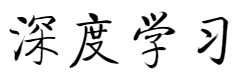
\includegraphics[]{proposal-fig-qiti.png}
    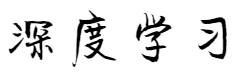
\includegraphics[]{proposal-fig-jinglei.png}

    Figure 1. Same characters in different fonts.\\The second font is more uneven and compact.
\end{center}


\section{Related Works}
\subsection{Image Style Transfer Using CNN}
It is an algorithm that can separate and recombine the image content and style of natural images. A Convolutional Neural Network is trained to extract high level image information and produce new images of high perceptual quality that combine the content of an arbitrary photograph with the appearance of specified artworks. This work proves the feasibility of using CNN for image style transfer.

\subsection{StyleGAN}
StyleGAN is a GAN architecture with a style-based generator that receives additional inputs to adjust the style. It leads to an automatically learned, unsupervised separation of high-level attributes and stochastic variation in the generated images, and it enables intuitive, scale-specific control of the synthesis.
\\
Unlike the traditional CNN decoder, StyleGAN adds an adaptive instance normalization (AdaIN) function to each convolution layer, where additional information is introduced to adjust the style.
\\
StyleGAN has an inspiring feature as known as Style Mixing, which allows the generator to mix the basic features (skeleton) of one image with the advanced features (style) of another image by applying their latent codes at different levels.

\subsection{SKFont: skeleton-driven Korean font generator}
With a limited sample of Korean characters, this research investigates the topic of font synthesis using an end-to-end conditional deep adversarial network. Only 114 samples are required for the SKFont model to generate the remaining characters in the same font style. This is accomplished in three steps.

\begin{enumerate}
\item Generate complete target font characters by observing 114 target characters.
\item Extract the structures of the synthesized characters obtained from the first step.
\item Transfer the style of the target font onto these learned structures.
\end{enumerate}
This approach resolves flaws such as blurriness, breakage, and a lack of delicate shape and style delivery.


\subsection{Word Level Font-to-Font Image Translation}
They propose a network that can convert any printed text image's font style from its existing font to the desired font. Since the network is trained end-to-end for the complete word images, it eliminates the necessary pre-processing steps, like character segmentation. To learn the one-to-many mapping function, they apply conditional setting. It also aids in the consistency of the final images after concatenating the target font's generated image patches. The majority of previous image translation research has been done on square pictures. This is the first architecture of its sort that can accommodate images of varied widths.



\section{Dataset}
The dataset includes $32 \times 32$ images of common characters converted from different font files. System fonts such as Brush Script MT and Segoe Script can be used at the beginning. More handwritten fonts will be collected if necessary. We plan to start with English characters and numbers, and then introduce Chinese characters.

\section{Model}
We first plan to build a Generative Adversarial Network, which consists of a Style-based generator with CNN encoder and a 5-layer conditional discriminator. The input and output are both $32 \times 32$ single-channel (black and white) images.

\\
On each training epoch, two images of different fonts are fed into the model. The one providing the skeleton will be used for the lower part of the decoder, and the one providing the style will be used for the upper part.
\begin{center}
    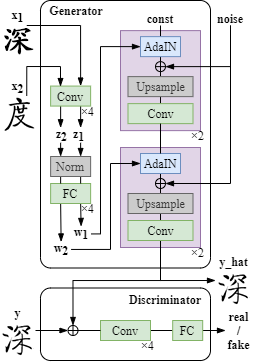
\includegraphics[]{plan-fig-model.png}

    Figure 2. Rough structure of our generator\\and discriminator. The generator includes\\a 4-layer CNN encoder, a 4-layer Mapping\\Network and a 4-layer Synthesis Network\\(CNN decoder with AdaIN).
\end{center}
Denote an image of character $i$ and font $F_k$ by $F_k[i]$. For each time, the generator takes a pair of images $(x_1=F_0[i], x_2=F_k[j])$ and outputs an image $\hat{y}$ with skeleton of $x_1$ and style of $x_2$. The discriminator differs the output from the groundtruth image $y=F_k[i]$. Font $F_0$ should have clear skeletons, and can be the same whenever training or testing.

Stylegan should train an autoencoder first, then mix input x1 and x2 together to see if we can get y. However, this method is not directly training $f(x1,x2)=y$, and the controllable is relatively poor. So we also use a directly trained pix2pix model to compare the effect with the Stylegan.


\section{Training Details}
please introduce the loss funtion(lsgan loss and wgan loss), parameters definition, training routine and anything you think appropriate.

\section{Hyperparameter Selection}
We did hyperparameter selection on some training parameters: the learning rate, batch size, iteration number, the $gdrate$, and the gan loss function. Our default setting is lr = 0.01, batch size = 8, iteration number = 2000,  $gdrate$ = 10, gan loss = lsgan loss.

We decided to change 1 hyperparameter a time which are 6 models totally. The measurement of these models are the mse loss of $y true$ and $y hat$ we generate. We compute the loss every epoch for validation dataset. Here is a figure of the loss per sample among epochs.


\begin{center}
    \includegraphics[width=.5\textwidth]{MSEloss among epochs.png}

    Figure 3. MSE Loss among epochs for 6 different models.
\end{center}

From this figure, we can found that using lsgan loss funtion and ... could make the model perform better.

\section{Preliminary Results}
We have obtained results from the 6 hyperparameter selection experiments.

For the default setting, our results are shown below. the first column is the font that providing the style(font2), for each font, we chose 3 samples from test dataset. In each small sample result, from left to right, are $x_2$ in font that providing the skeleton(font1), $x_1$ in font1, $x_2$ in font2, $x_2$ in font2, the $x_2$ in font2 we generated. So we can regard the right 2 as $y true$ and $y hat$.

\begin{center}
    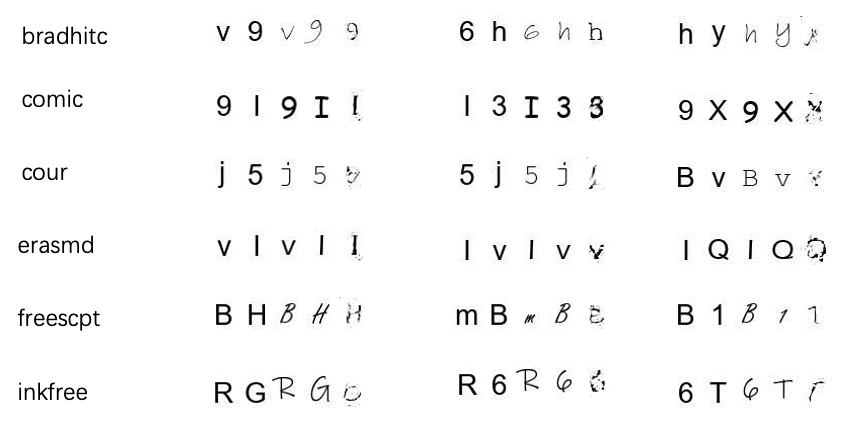
\includegraphics[width=.5\textwidth]{lr_0.01_batchsize_8_g_d_rate_10_loss_lsgan.png}

    Figure 4. Results under lr=0.01 batchsize=8 $gdrate$=10 loss=lsgan.
\end{center}

For experiment 2, we enlarge the leaning rate to 0.03. For experiment 3, we set 50 as the batch size and the iteration number changed accordingly to 320. For experiment 4, we set 100 as the batch size and the iteration number changed accordingly to 160. For experiment 5, we smaller the $gdrate$ to 1. For experiment 6, we switch the loss function to wgan loss. These results are shown below. We can observe that the wgan loss model has not learned the style but just the skeleton.


\begin{center}
    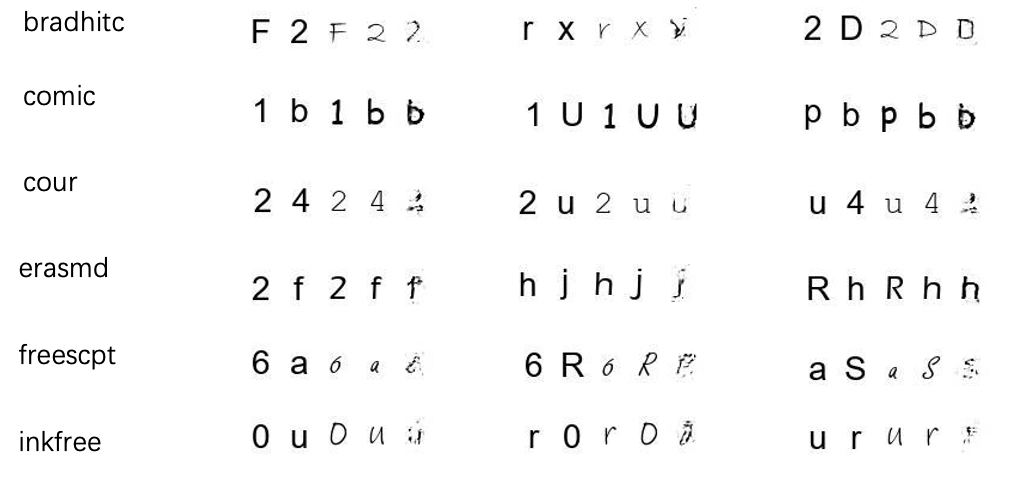
\includegraphics[width=.5\textwidth]{lr_0.03_batchsize_8_g_d_rate_10_loss_lsgan.png}

    Figure 5. Results under lr=0.03 batchsize=8 $gdrate$=10 loss=lsgan.
\end{center}

\begin{center}
    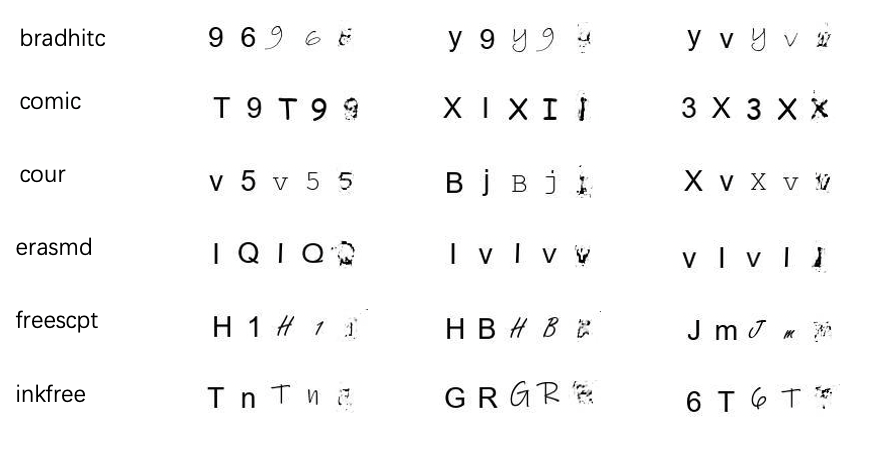
\includegraphics[width=.5\textwidth]{lr_0.01_batchsize_50_g_d_rate_10_loss_lsgan.png}

    Figure 6. Results under lr=0.01 batchsize=50 $gdrate$=10 loss=lsgan.
\end{center}

\begin{center}
    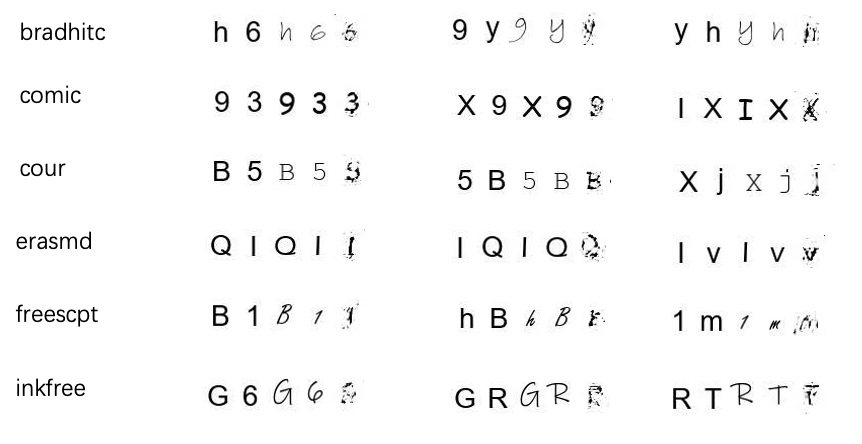
\includegraphics[width=.5\textwidth]{lr_0.01_batchsize_100_g_d_rate_10_loss_lsgan.png}

    Figure 7. Results under lr=0.01 batchsize=100 $gdrate$=10 loss=lsgan.
\end{center}

\begin{center}
    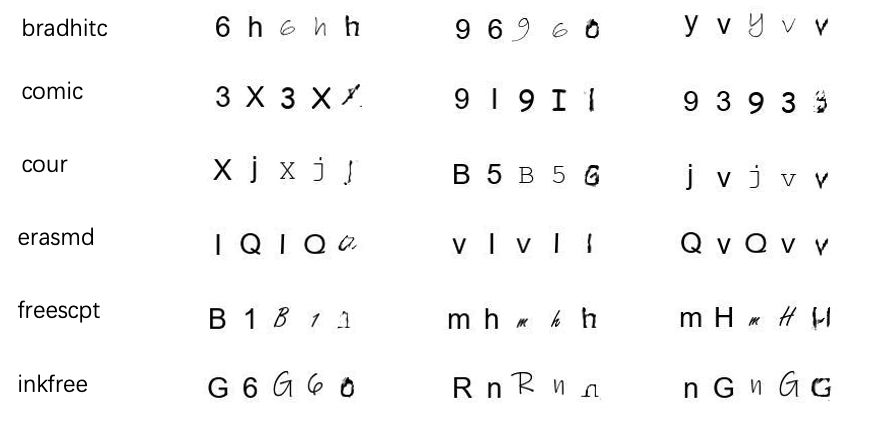
\includegraphics[width=.5\textwidth]{lr_0.01_batchsize_8_g_d_rate_1_loss_lsgan.png}

    Figure 8. Results under lr=0.01 batchsize=8 $gdrate$=1 loss=lsgan.
\end{center}

\begin{center}
    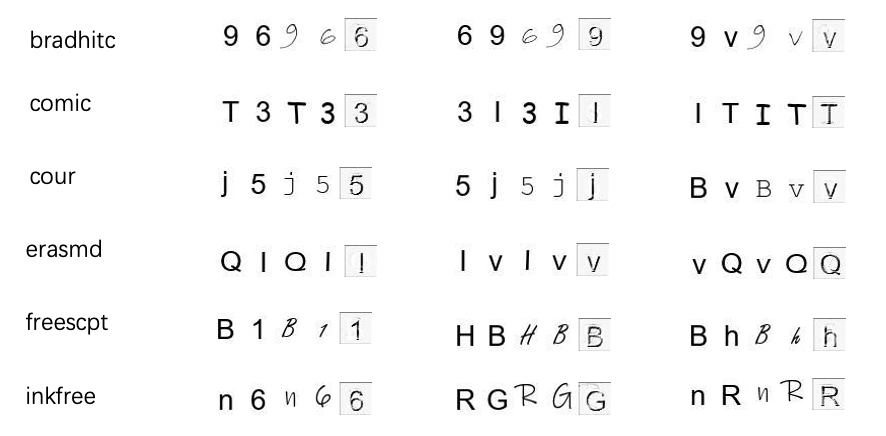
\includegraphics[width=.5\textwidth]{lr_0.01_batchsize_8_g_d_rate_10_loss_wgan.png}

    Figure 9. Results under lr=0.01 batchsize=8 $gdrate$=10 loss=wgan.
\end{center}



\section{Possible Challenges and Concerns}

\section{Remaining Work}

\section{Anticipated Outcomes}
To be specific, the generator is expected to generate a new character image which mixes the structure of one input and the style of another. The discriminator should be able to tell whether a pair of images describe the same character and belong to the same font.
\\
Therefore, a well-trained generator can generate images of any character $i$ in the style of any font $F_k$. If we input a handwritten character image $x_2=F_{new}[j_0]$ repeatly with all common characters $x_1\in F_0$, we'll get a new handwritten font $F_{new}$.

\section{Challenges and Concerns}
\begin{itemize}
    \item The training process can be disoriented with two independent input variables. It might be better to start with an autoencoder.
    \item The CNN encoder block is shared by two independent datapaths and provides relatively more static functions, which means it can be pre-trained rather than roughly training the whole generator together.
    \item The skeleton provider, $F_0[i]$, also plays the role of identifier. If our generator have the ability to remember the skeleton of all characters, we can remove $x_1$ and input one-hot character codes into the decoder instead.
    \item Notice that fonts are stored in the form of vector graphs of quadratic Bezier curves. The final model should include a image trace module to output vector graphs.
\end{itemize}

\section{Reference}
\smallskip \noindent
Leon, A. G., Alexander, S. E., and Matthias, B. 2016. Image Style Transfer Using Convolutional Neural Networks. \textit{CVPR}, pp. 2414-2423.

\smallskip \noindent
Tero, K., Samuli, L., and Timo, A. 2019. A Style-Based Generator Architecture for Generative Adversarial Networks. \textit{CVPR}, abs/1812.04948.

\smallskip \noindent
Ko, D. H., Hassan, A. U., Suk, J., \& Choi, J. 2021. SKFont: skeleton-driven Korean font generator with conditional deep adversarial networks. \textit{International Journal on Document Analysis and Recognition (IJDAR)}, 1-13.

\smallskip \noindent
Bhunia, A. K., Bhunia, A. K., Banerjee, P., Konwer, A., Bhowmick, A., Roy, P. P., \& Pal, U. 2018. Word level font-to-font image translation using convolutional recurrent generative adversarial networks. \textit{ICPR} (pp. 3645-3650).



\bibliography{proposal-reference.bib}
\bibliographystyle{aaai}
\end{document}